\documentclass[12pt]{article}
\usepackage{url}
\usepackage{graphicx}
\usepackage{verbatim}
\usepackage[answerdelayed]{exercise}

\setlength{\ExerciseSkipBefore}{1em}
\setlength{\ExerciseSkipAfter}{1em}
\renewcommand{\ExerciseHeader}{\noindent\textbf{\normalsize\ExerciseName\space\ExerciseHeaderNB\quad}\par}
\renewcommand{\AnswerHeader}{\noindent\textbf{Answer to \normalsize\ExerciseName\space\ExerciseHeaderNB\quad}\par}

\title{Stats exam 2014}
\author{Guillaume Filion}

\begin{document}

\maketitle

Please submit your answers by email to
\texttt{guillaume.filion@gmail.com} before the deadline. Each
question is worth 1 point. Every fraction of 24 hours passed
the deadline will be penalized by 2 points. You are encouraged
to work in group on these exercises.
You can submit a joint answer sheet and will receive the same
grade as your team members. In this case, indicate the name of
all the students participating to the work.

The answers will be posted online at the address below. \par
\noindent \url{www.genomearchitecture.com/static/misc/statsexam_answers_2014.pdf}

\section{Course questions}

\begin{Exercise}[label={exo1}]
  What are the main steps of a test?
\end{Exercise}
\begin{Answer}[ref={exo1}]
  \begin{enumerate}
    \item State the null hypothesis.
    \item Choose a statistic.
    \item Compute the null distribution.
    \item Compare the observed value of the stastic to the null.
  \end{enumerate}
\end{Answer}

\begin{Exercise}[label={exo2}]
  What is the p-value of a test?
\end{Exercise}
\begin{Answer}[ref={exo2}]
  The probability that the statistic is more extreme, given that
  the null hypothesis is true.
\end{Answer}

\begin{Exercise}[label={exo3}]
  What is the power of a test?
\end{Exercise}
\begin{Answer}[ref={exo3}]
  The probability of rejecting the null hypothesis.
\end{Answer}

\begin{Exercise}[label={exo4}]
  How can you increase the power of a test?
\end{Exercise}
\begin{Answer}[ref={exo4}]
  By increasing the level or by increasing the sample size.
\end{Answer}

\begin{Exercise}[label={exo5}]
  What is the statistic of the $t$-test?
\end{Exercise}
\begin{Answer}[ref={exo5}]
  The effect size.
\end{Answer}

\section{Problem}

  An insecure implementation of a password-protected acess
  is to compare letter by letter the text enterred by the
  user to the real password, and to deny access as soon
  as a different letter is found. This is insecure because
  it opens a possibility for \textit{a timing attack}, which
  is an attempt to hack a password by measuring the time it
  takes for the computer to respond.

  \url{http://en.wikipedia.org/wiki/Timing_attack}

  Suppose that my real password is \texttt{kotiki125}. If
  the hacker enters \texttt{abcdefg}, the insecure method will
  deny access immediately after comparing the first letter
  because \texttt{a} is different from  \texttt{k}. But
  if the hacker enters \texttt{kotiki123}, this method
  will deny access upon comparing the 9-th letter, which will
  take roughly 9 times as long. With this information, the
  hacker could deduce that the first 8 letters of
  \texttt{kotiki123} are correct.

  The idea of a timing attack is to try all the letters
  one by one and measure the time it takes for the computer
  to respond. Every time a letter matches the password, the
  response time will be slightly slower. By repeating the
  process, the password can be decrypted completely.

\begin{Exercise}[label={exo6}]
  Assume that there are 64 valid password letters
  (small letters, capital letters, numbers, \texttt{\_} and
  \texttt{\~}, and that you want to decrypt a password
  generated at random. You enter a text. What is the
  probability that the first letter matches the password?
  What is the probability that the first 3 letters match
  the password?
\end{Exercise}
\begin{Answer}[ref={exo6}]
  $\left(\frac{1}{64}\right)^3 \approx 3.8 \cdot 10^{-6}$
\end{Answer}

  Based on previous measurements, you know that the
  time to compare two letters is 10 ns. In addition, for
  every letter comparison, there is a random overhead due
  to other processes running on the server. This overhead
  has an exponential distribution with rate 0.125 ns$^{-1}$.

  \begin{Exercise}[label={exo7}]
  The function \texttt{rexp(8, rate=.125)} in \texttt{R}
  generates a random sample of size 8 drawn from an
  exponential distribution with rate 0.125 ns$^{-1}$.
  How to generate a random sample of size 8 representing
  the response time of the server when the first letter of
  the text does not match the password?
\end{Exercise}
\begin{Answer}[ref={exo7}]
  \texttt{10+rexp(8, rate=.125)}
\end{Answer}

  You have entered the text \texttt{aaaaaaaa} 8 times
  and have observed the following response times (in ns)
  23.0, 15.7, 21.4, 12.8, 13.3, 21.3, 38.2, 15.4.

  \begin{Exercise}[label={exo8}]
  Do you think that the first letter of the password is
  \texttt{a}? Quantify your certainty. Before you set up 
  a complicated statistical test, look at the numbers
  carefully.
\end{Exercise}
\begin{Answer}[ref={exo8}]
  If the first letter is \texttt{a}, there will be at
  least 2 letter comparisons, which takes at least 20 ns.
  Since at least one of the numbers is lower than 20 ns,
  this cannot be the case.
\end{Answer}

  You know that the password starts with \texttt{wy6qU}.
  You now enter \texttt{wy6qUaaaaa} 8 times and obtain
  the following response times (in ns)
  122.0, 83.8, 71.4, 136.6, 93.6, 88.1, 84.1, 123.0

  In \texttt{R} you can compute the sum of 6 exponential
  random variables with rate 0.125 ns$^{-1}$ by using
  \texttt{sum(rexp(6, rate=.125)}. Similarly, you can
  generate a sample of size 8 representing the response
  time of the server if the 6-th letter does not match
  by using \texttt{replicate(8,60+sum(rexp(6,rate=.125)))}.

  \begin{Exercise}[label={exo9}]
  Using this information, design a statistical test to
  know whether the 6-th letter of the password is \texttt{a}.
  Quantify your certainty.
\end{Exercise}
\begin{Answer}[ref={exo9}]
  \begin{enumerate}
    \item Ho: the 6-th letter is not \texttt{a}
    \item The statistic is the minimum response time.
    \item To identify the null distribution we do the following
      in \texttt{R}.

\begin{verbatim}
mins <- rep(NA, 10000)
for (i in 1:10000) {
  mins[i] <- min(replicate(8,60+sum(rexp(6,rate=.125))))
}
\end{verbatim}

    \item To compare the sample to the null distribution we do the
      following.

\begin{verbatim}
hist(mins, breaks=50)
abline(v=71.4, col=2)
mean(mins < 71.4) # 0.0264
\end{verbatim}

  \end{enumerate}

  We get the graphical results shown below. In only 2.6\% of
  the cases we get a lower minimum value out of 8. This means
  that the minimum value for our sample is \textit{low} and that
  we should \textit{not} reject the null hypothesis, because
  if the null hypothesis is true, we expect the minimum value
  to be low. This is a special case where it makes sense to
  use a one-sided test and put all the rejection on the right
  side of the distribution, which corresponds to our intuition
  in the case that the null hypothesis is false.

  \centerline{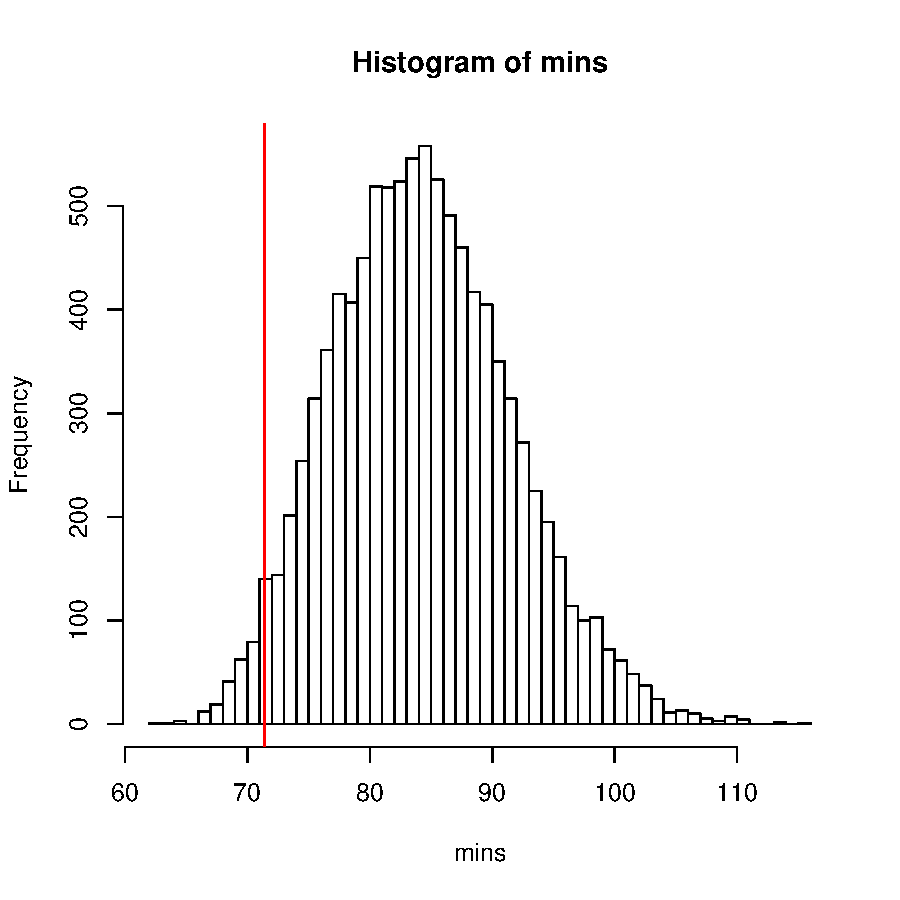
\includegraphics[scale=0.5]{mins.pdf}}

  This exercise is interesting because several choices are
  possible for the statistic. We could as well take the average
  instead of the minimum, but Exercise 8 suggests that taking
  the minimum contains more information. If we take the average,
  the null distribution is different, and also the power. Also,
  it is one of a few cases where the rejection \textit{should}
  be one-sided because the alternative hypothesis is simple
  (\textit{i.e.} not composite), if the null hypothesis is
  false, the response time will be longer (and not either
  longer or shorter). Also note that the null hypothesis cannot
  be that the 6-th letter is \texttt{a} because this does not
  allow to compute the null distribution (the distribution then
  depends on whether the 7-th and further letters are guessed
  correctly).

\end{Answer}

\begin{Exercise}[label={exo10}]
  What is the power of your test?
\end{Exercise}
\begin{Answer}[ref={exo10}]
  In this case, it makes sense to compute the power when the 6-th
  letter is \texttt{a} (the null hypothesis is false) and the
  7-th letter is wrong. In this case, the distribution of
  the sample will be \texttt{replicate(8,70+sum(rexp(7,rate=.125)))}.

\begin{verbatim}
mins2 <- rep(NA, 10000)
for (i in 1:10000) {
   mins2[i] <- min(replicate(8,70+sum(rexp(7,rate=.125))))
}
threshold <- quantile(mins, 0.95) # 97.00
mean(mins2 > threshold) # 0.63
\end{verbatim}

  So when the null hypothesis is false, we reject it 63\% of
  the time, which is the power of the test. Note that if the 7-th
  letter is correct, the response time will be longer and the
  rejection will happen more than 63\% of the time, so this
  number represents the minimum power.
  
  If the queries are free
  (in terms of time or risk for the hacker), it makes sense
  to do more than 8 per letter in order to raise the power close
  to 1.0. Otherwise, it is a matter of computing the cost/benefit
  ratio for the hacker keeping in mind that the hacker would have
  only 63\% chance of identifying the right letter with 8 queries.
  


\end{Answer}

\cleardoublepage
\shipoutAnswer

\end{document}
